\pagestyle{fancy}
\setlength{\headheight}{16pt}
\fancyhead{} % clear all header fields
\fancyhead[L]{\textbf{TAM 514 Homework 1}}
\fancyhead[C]{Songyuan Cui}
\fancyhead[R]{\textbf{Spring 2025}}
\fancyfoot{} % clear all footer fields
\fancyfoot[C]{\thepage}

\begin{problem}
    \begin{wrapfigure}{r}{0.5\textwidth}
        \vspace{-0.35cm}
        \centering
        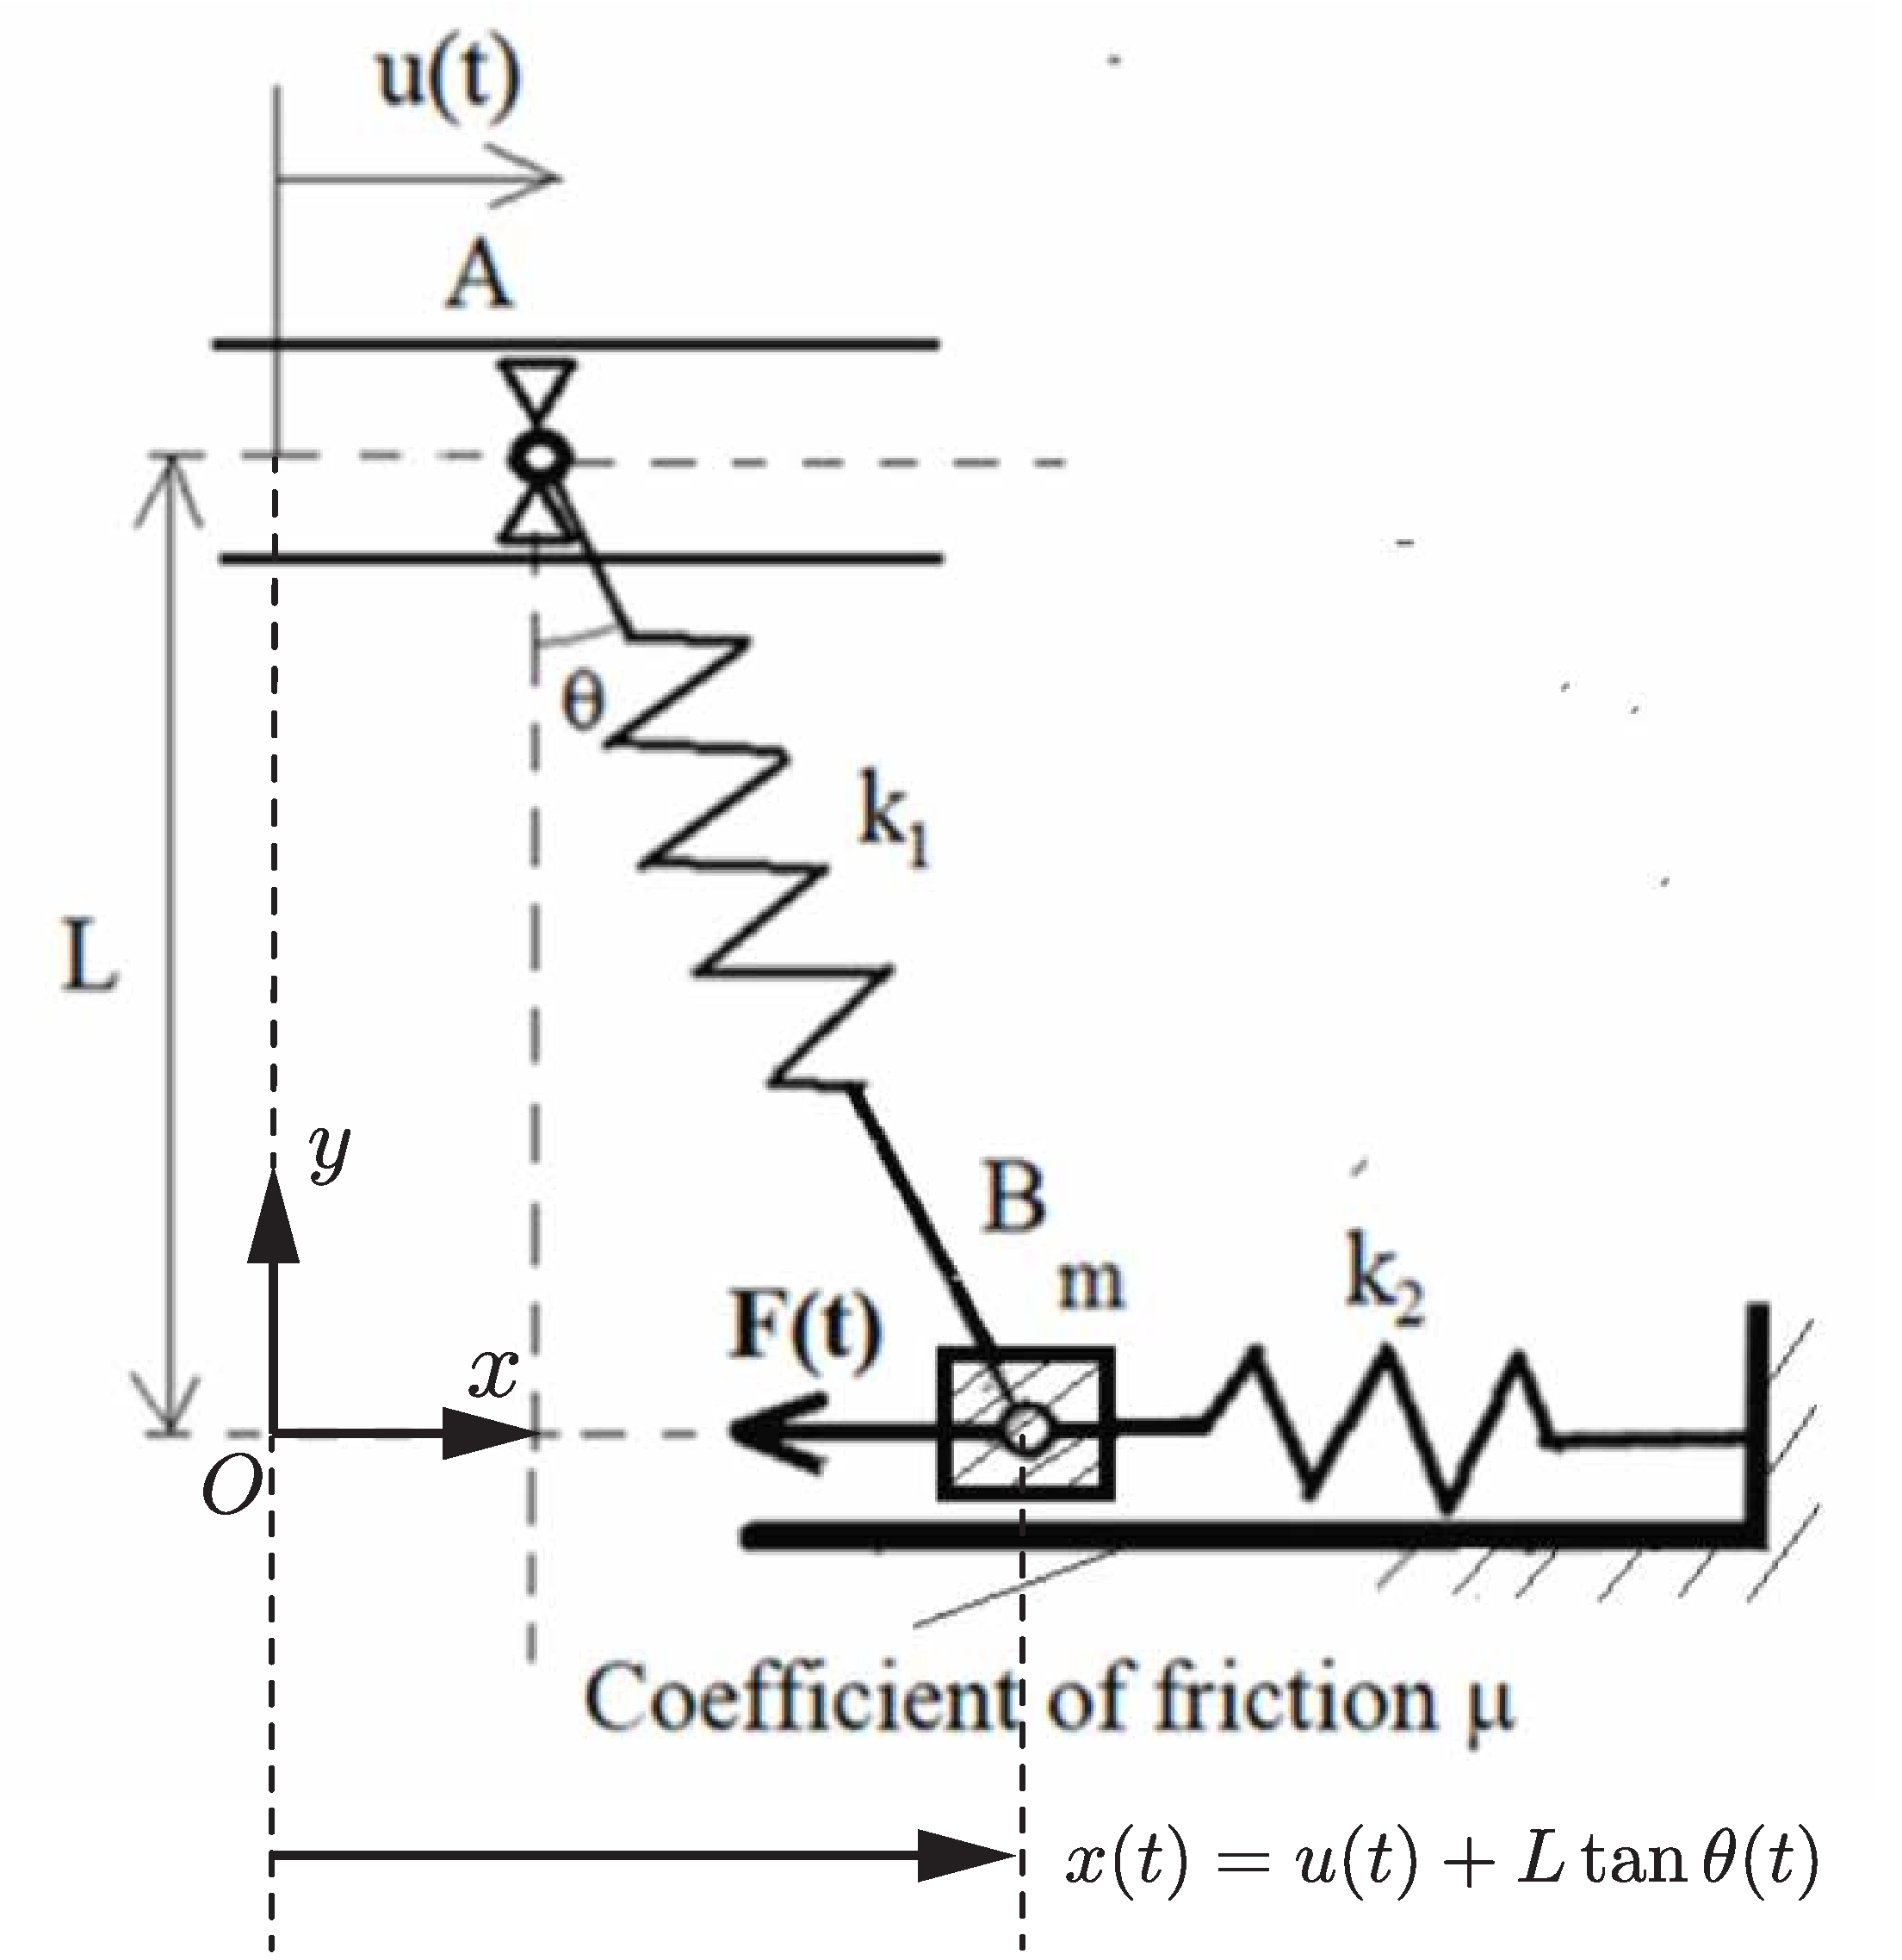
\includegraphics[width=0.8\linewidth]{homework/hw1/assets/hw1_p1_annotated.pdf}
    \end{wrapfigure}
    \textbf{1. (50 pts)} Consider the mechanical system shown. 
    Pivot A slides horizontally with a \ul{prescribed} displacement $u(t)$, and mass B is also restricted to more horizontally on a rough base. 
    The system is in static equilibrium (and the springs are unstretched) when $\theta(t) = u(t) = 0$. 
    The only mass of the system is $m$, and the coefficient of friction of the rough base where mass $m$ is sliding is $\mu$. 
    A horizontal force $\bt{F}(t)$ is applied to the mass. 
    Gravity is included.
    \begin{enumerate}[(i)]
        \item {
            How many degrees of freedom (DOFs) does this system have?
        }
        \item {
            Derive the equation(s) of motion of this system using Lagrange's equations.
        }
    \end{enumerate}
\end{problem}

\begin{enumerate}[(i)]
\item { % 1(i)
    This system has \fbox{one} degrees of freedom $\theta(t)$. 
    With $u(t)$ prescribed, $\theta$ alone defines the entire system.
}
\item {
    We define a coordinate system with the origin located at $u = 0$, as shown in the figure.
    For convenience, the displacement of the mass $m$ from the origin is defined as 
    \begin{equation}\label{eqn:hw1_p1_x}
        x(t) = u(t) + L \tan \theta(t)
    \end{equation} 
    which we note is not an independent variable. 
    The equation of motion is derived through the extended Hamilton's principle:
    \begin{equation}\label{eqn:hw1_p1_hamilton}
        0 = \int_0^T \Pi[\theta](t) dt = \int_0^T (\delta K - \delta V + \delta R) dt 
    \end{equation}
    where $K$ is the kinetic energy, $V$ is the (elastic) potential energy, and $R$ is the work done by the external force. 
    The kinetic energy and potential energy are given by 
    \begin{equation}
        K = \frac{1}{2} m \dot{x}^2, ~~~~ V = \frac{1}{2} k_1 {\left(\frac{L}{\cos\theta} - L\right)}^2 + \frac{1}{2} k_2 x^2
    \end{equation}
    The work done by the external force is more easily formulated via its variation as the virtual work $\delta R = F \delta x$, where $F$ is defined to point in the \emph{positive $x$ direction}, and $\delta x$ can be expressed as a function of $\delta \theta$ 
    \begin{equation}
        \delta x = L \sec^2\theta \delta \theta
    \end{equation}
    Furthermore, the action via kinetic and potential energy are ($\delta x = 0$ at $t=0$ and $t=T$). 
    \begin{subequations}
    \begin{equation}
    \begin{aligned}
        \int_0^T \delta K dt &= \int_0^T m \dot{x} \delta \dot{x} dt = - \int_0^T m \ddot{x} \delta x dt \\
        &= - \int_0^T m \ddot{x} L \sec^2\theta \delta \theta dt
    \end{aligned}
    \end{equation}
    \begin{equation}
    \begin{aligned}
        \int_0^T \delta V dt &= \int_0^T \left[ k_1 L^2  \left( \sec\theta - 1\right) \sec\theta \tan\theta \delta \theta + k_2 x \delta x \right] dt \\
        &= \int_0^T \left[ k_1 L^2  \left( \sec\theta - 1\right) \sec\theta \tan\theta + k_2 x L \sec^2\theta \right] \delta\theta dt
    \end{aligned}
    \end{equation}
    \end{subequations}
    Substituting back into \cref{eqn:hw1_p1_hamilton} and leveraging variational principle (setting the integrand to zero and cancel $L\sec^2\theta$) yields the equation of motion:
    \begin{equation}\label{eqn:hw1_p1_eom}
        \boxed{m\ddot{x} + k_1 L (\tan\theta - \sin\theta) + k_2 x = F}
    \end{equation}
    where $x(t)$ is given in \cref{eqn:hw1_p1_x} and 
    \begin{equation}
    \begin{aligned}
        \ddot{x}(t) &= \ddot{u}(t) + L\frac{d^2}{dt^2} \left[ \tan\theta(t) \right] \\
        &= \Aboxed{\ddot{u}(t) + L \sec^2\theta(t) \ddot{\theta}(t) + 2L \sec^2\theta(t) \tan\theta(t) {\dot{\theta}(t)}^2}
    \end{aligned}
    \end{equation}

    \begin{errata}
    The provided solution failed to account for the friction forces at the surface. 
    To correct this, we first assume a gravitational constant $g$ and that the mass $m$ is sufficiently large for there to always be a contact force between the mass and the surface.
    The friction can then be incorporated into the external work, in which 
    \begin{equation}
        \delta R = F \delta x - \mu \left[m g - k_1 L \left( \sec\theta - 1\right) \cos\theta\right] \sign{\dot{x}} \delta x
    \end{equation}
    and \cref{eqn:hw1_p1_eom} is therefore modified to 
    \begin{equation}
        m\ddot{x} + k_1 L (\tan\theta - \sin\theta) + k_2 x = F - \mu \left[m g - k_1 L \left( 1 - \cos\theta \right) \right] \sign\left(\dot{u} + L \sec^2\theta \dot{\theta} \right)
    \end{equation}
    \end{errata}
}
\end{enumerate}


\begin{problem}
    \begin{wrapfigure}{r}{0.45\textwidth}
        \vspace{0.75cm}
        \centering
        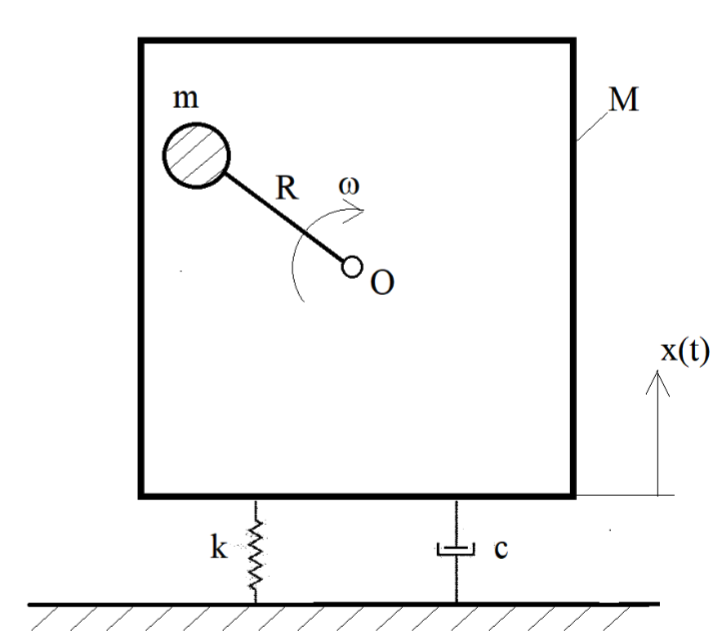
\includegraphics[width=0.9\linewidth]{homework/hw1/assets/hw1_p2.png}
    \end{wrapfigure}
    \textbf{2. (50 pts)} Consider a machine of mass $M$ with a rotating imbalance produced by a mass $m$ rotating with frequency $\omega$ about an axis orthogonal to the plane and positioned at a radius $R$ from the axis of rotation. 
    At $t = 0$ the mass $m$ is at its top vertical position. 
    We assume that the machine is suspended by a spring $k$ in parallel to a viscous damper $c$, and is constrained to move in the vertical direction. 
    Gravity is ignored.

    \begin{enumerate}[(i)]
        \item {
            Show that the vertical response of the machine with respect to an inertial frame is governed by the equation:
            \begin{equation}
                (M + m) \ddot{x}(t) + c \dot{x}(t) + k x(t) = m R \omega^2 \cos \omega t
            \end{equation}
        }
        \item {
            Compute the steady state response $x(t)$ of the machine.
        }
        \item {
            If there is no damping ($c = 0$) when will resonance occur?
        }
    \end{enumerate}
\end{problem}

\begin{enumerate}[(i)]
\item { % 2(i)
    Assuming $x(t) = 0$ corresponds to the neutral position of the spring $k$, the potential energy of the system is $V = kx^2 / 2$.
    The instantaneous velocity vector of $m$, with respect to an inertial frame, is 
    \begin{equation}
        \bv{v} = \omega R \cos{\omega t} \hat{\bv{i}} + \left(\dot{x} - \omega R \sin{\omega t}\right) \hat{\bv{j}}
    \end{equation}
    where in the figure, $\hat{\bv{i}}$ points to the right and $\hat{\bv{j}}$ points upwards.
    Thus, the total kinetic energy of the system is 
    \begin{equation}
    \begin{aligned}
        K &= \frac{1}{2} M \dot{x}^2 + \frac{1}{2} m \left[ {\left(\omega R \cos{\omega t} \right)}^2 + {\left( \dot{x} - \omega R \sin{\omega t} \right)}^2 \right] \\
        &= \frac{1}{2} (M + m) \dot{x}^2 + \frac{1}{2}m\omega^2 R^2 - m \omega R \dot{x} \sin{\omega t}
    \end{aligned}
    \end{equation}
    With respect to the displacement variation $\delta x$, we regard the damping force as a generalized force $F_d(t) = -c \dot{x}(t)$ where, assuming $c \geq 0$, the negative sign implies the damping force counteracts the motion.
    Directly applying the generalized Euler-Lagrange equation with Lagrangian $\mathcal{L} := K - V$, 
    \begin{equation}
    \begin{aligned}
        \frac{d}{dt} \left( \frac{\partial \mathcal{L}}{\partial \dot{x}} \right) - \frac{\partial \mathcal{L}}{\partial x} = F_d(t), ~~~~ &\Rightarrow ~~~~ \frac{d}{dt}\left[(M+m)\dot{x} - m \omega R \sin\omega t\right] + kx = -c\dot{x} \\
        &\Rightarrow ~~~~ \Aboxed{(M + m) \ddot{x}(t) + c \dot{x}(t) + k x(t) = m \omega^2 R \cos \omega t}
    \end{aligned}
    \end{equation}
    hence concludes the proof. 
}
\item { % 2(ii)
    We can find a periodic orbit (limit cycle) by creating an ansatz 
    \begin{equation}
        \boxed{\bar{x}(t) = A \cos \omega t + B \sin\omega t}.
    \end{equation}
    Substituting into the equation of motion and matching the coefficients for $\cos\omega t$ and $\sin\omega t$, respectively, yields a linear system 
    \begin{equation}
        \begin{bmatrix}
            k - (M+m)\omega^2 & - \omega c \\
            \omega c & k - (M+m)\omega^2 
        \end{bmatrix} 
        \begin{bmatrix}
            A \\ B
        \end{bmatrix} = 
        \begin{bmatrix}
            m R \omega^2 \\ 0
        \end{bmatrix}
    \end{equation}
    For conciseness, we denote the determinant of the imposing matrix as 
    \begin{equation}\label{eqn:hw1_p2_det}
        \Delta := \det \begin{bmatrix}
            k - (M+m)\omega^2 & - \omega c \\
            \omega c & k - (M+m)\omega^2
        \end{bmatrix} = k^2 + \omega^2 c^2 + {(M+m)}^2 \omega^4 - 2k(M+m)\omega^2.
    \end{equation}
    The coefficients $A, B$ are obtained by inverting the system,
    \begin{equation}
       \boxed{ A = \frac{1}{\Delta} \left[k - (M+m) \omega^2 \right](m\omega^2 R), ~~~~ B = \frac{1}{\Delta} \left( m c R \omega^3 \right) }
    \end{equation}
}
\item { % 2 (iii)
    In the absence of damping ($c = 0$), resonance occurs when $\Delta = 0$ (i.e.~the system is singular).
    This implies 
    \begin{equation}
        k - (M + m) \omega^2 = 0 ~~~~ \Leftrightarrow ~~~~ \boxed{\omega = \sqrt{\frac{k}{M+m}}}.
    \end{equation}

}
\end{enumerate}

\begin{problem}
    \begin{wrapfigure}{r}{0.4\textwidth}
        \vspace{-0.5cm}
        \centering
        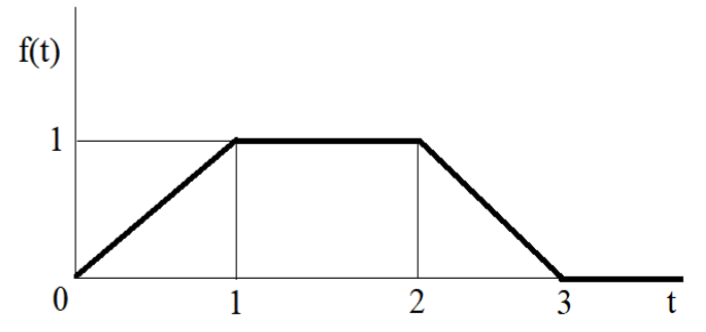
\includegraphics[width=0.82\linewidth]{homework/hw1/assets/hw1_p3.png}
    \end{wrapfigure}
    \textbf{3 (50pts)} Consider the following forced oscillator,
    \begin{equation}
        \ddot{x}(t) + x(t) = f(t), ~~ x(0) = 1, ~~ \dot{x}(0) = -2
    \end{equation}
    where $f(t)$ is shown in the figure. Compute the response
    using Laplace transform.  
\end{problem}
Denote the Laplace transform of $f(t)$ as 
\begin{equation}
    X(s) = \mathcal{L}[x(t)](s) := \int_0^\infty x(t) e^{-st} dt.
\end{equation}
It is straightforward to prove the following properties of Laplace transform that shall prove useful:
\begin{align}
    \mathcal{L}[\dot{x}(t)](s) &= sX(s) - x(0) \label{eqn:hw1_p3_lxdot} \\
    \mathcal{L}[\ddot{x}(t)](s) &= s^2 X(s) - sx(0) - \dot{x}(0) \label{eqn:hw1_p3_lxddot}  \\
    \mathcal{L}[x(t-t_0) H(t-t_0)](s) &= e^{st_0} X(s) \label{eqn:hw1_p3_lxshift} 
\end{align}
where $H(t)$ is the Heaviside step function. 
\Cref{eqn:hw1_p3_lxdot,eqn:hw1_p3_lxddot} are derived by integrating by parts, and \cref{eqn:hw1_p3_lxshift} is easily proved by a change of variable such as $\tau = t - t_0$.

One easy way to compute the Laplace transform of the forcing function $f(t)$ is to replace its piecewise nature with Heaviside functions:
\begin{equation}
    f(t) = t - H(t-1)(t-1) - H(t-2)(t-2) + H(t-3)(t-3), ~~~~ t\geq 0.
\end{equation}
Since the Laplace transform of $t$ is simply $s^{-2}$ (integration by parts), we leverage \cref{eqn:hw1_p3_lxshift} to find the 
\begin{equation}
    F(s) = \mathcal{L}[f(t)](s) = \frac{1}{s^2} \left(1 - e^{-s} - e^{-2s} + e^{-3s}\right).
\end{equation}
Using \cref{eqn:hw1_p3_lxdot,eqn:hw1_p3_lxddot} and the initial conditions, the Laplace transform of the IVP is then 
\begin{equation}\label{eqn:hw1_p3_Xs}
    s^2 X(s) - s + 2 + X(s) = F(s) ~~~~ \Rightarrow ~~~~ X(s) = \frac{1}{s^2(s^2+1)} \left(1 - e^{-s} - e^{-2s} + e^{-3s}\right) + \frac{s-2}{s^2+1}.
\end{equation}
Notice the following,
\begin{equation}
    \frac{1}{s^2(s^2+1)} = \frac{1}{s^2} - \frac{1}{s^2+1}, ~~~~ \mathcal{L}[\cos t](s) = \frac{s}{s^2+1}, ~~~~ \mathcal{L}[\sin t](s) = \frac{1}{s^2+1},
\end{equation}
which is used to perform the inverse Laplace transform on $X(s)$ (\cref{eqn:hw1_p3_Xs}). 
\begin{equation}\label{eqn:hw1_p3_soln}
\begin{aligned}
    x(t) &= \mathcal{L}^{-1}[X(s)](t) \\
    &= (t + \cos t - 3\sin t) - H(t-1) (t - 1 - \sin(t - 1)) \\
    &~~~- H(t-2)(t - 2 - \sin(t-2)) + H(t-3)(t - 3 + \sin(t-3)).
\end{aligned}
\end{equation}
The solution is compared against numerical numerical in \cref{fig:hw1_p3_soln} with good quantitative agreement.

\begin{figure}
    \centering
    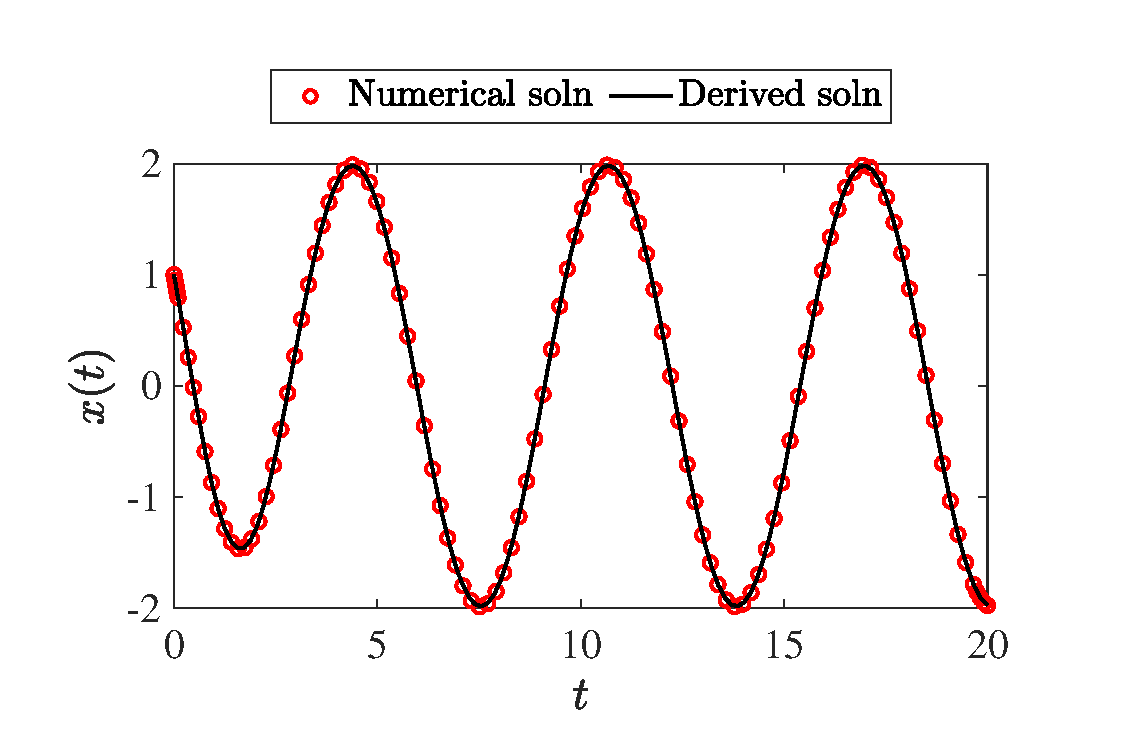
\includegraphics[width=0.5\linewidth]{homework/hw1/assets/hw1_p3_soln.pdf}
    \caption{The response $x(t)$ of the spring-mass system to the forcing function $f(t)$. The derived solution \cref{eqn:hw1_p3_soln} (black line) is compared against numerical solution (red circles) obtained via RK45 time integration.} 
    \label{fig:hw1_p3_soln}
\end{figure}

\begin{problem}
    \textbf{4. (50 pts)} Consider the system shown below. 
    Gravity is ignored, the only mass is the mass $m$ at position $B$, and the system is shown at the position of equilibrium. 
    We consider small rotations of this system about the pivot $O$.
    \begin{enumerate}[(i)]
        \item {
            Find the equation of motion.
        }
        \item {
            Determine the natural frequency $\omega_0$ and viscous damping ratio $\zeta$ of this system.
        }
        \item {
            Now select the relation that the system parameters should satisfy for the response to be overdamped, and in that case find the expression for the response for initial conditions $\theta(0) = \theta_0$ and $\dot{\theta}(0) = \omega_0$.
        }

    \end{enumerate}
    \begin{center}
        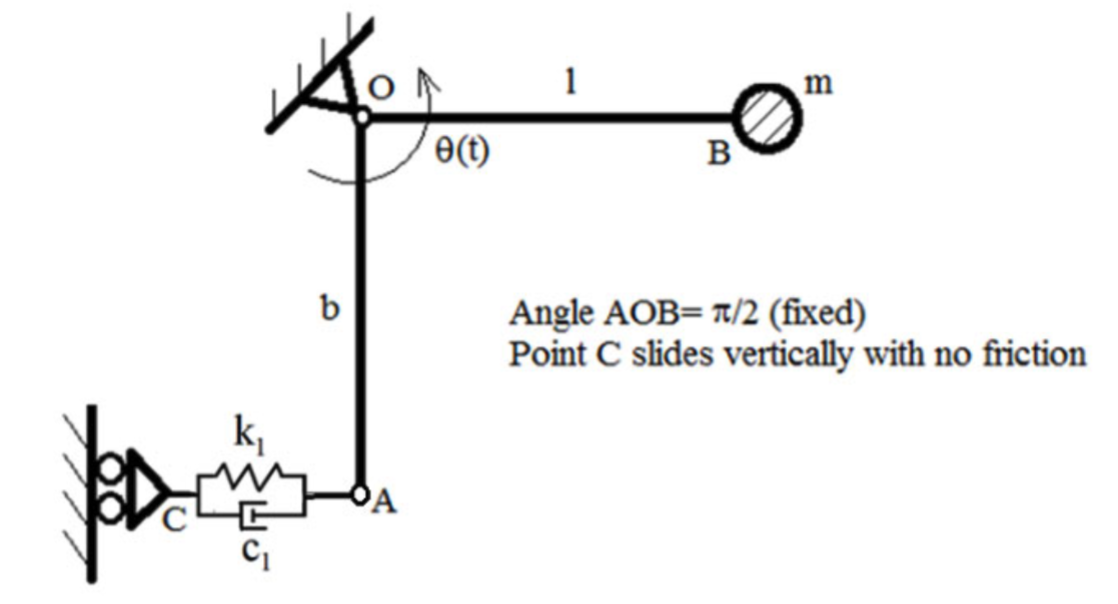
\includegraphics[width=0.5\linewidth]{homework/hw1/assets/hw1_p4.png}
    \end{center}
\end{problem}

\noindent\emph{Note: I cannot tell whether the length of the horizontal link is the letter `l' or the number `1'. I will henceforth assume it to be a known value `l' to be generic. Replace `l' in the solution with `1' if necessary. }

\begin{enumerate}[(i)]
\item {
    We begin by considering the full nonlinear problem. The displacement of point A from its reference position is 
    \begin{equation}
        \bv{x}_A(t) = b\sin\theta(t) \hat{\bv{i}} + b(1-\cos\theta(t)) \hat{\bv{j}},
    \end{equation}
    with $\hat{\bv{i}}$ pointing to the right and $\hat{\bv{j}}$ pointing upwards.
    For this problem, only the $\hat{\bv{i}}$ component and its velocity is of interest. 
    Hence we can compute the system's kinetic energy, potential energy, and the generalized force due to the dashpot damping: 
    \begin{equation}
    \begin{aligned}
        K &= \frac{1}{2} m l^2 \dot{\theta}^2, ~~~~ V &= \frac{1}{2} k_1 b^2 \sin^2 \theta, ~~~~ F_d = -c_1 b^2 \cos^2\theta \dot{\theta}
    \end{aligned}
    \end{equation}
    Here, $F_d$ is obtained by taking the variational derivative of the damping force with respect to $\delta \theta$:
    \begin{equation}
        F_d\delta \theta = -c_1 b \dot{\theta} \cos\theta \delta \left(b \sin\theta \right) = -c_1 b^2 \cos^2 \theta \dot{\theta} \delta \theta.
    \end{equation}
    Again, defining the Lagrangian $\mathcal{L} := K - V$ and using the generalized Euler-Lagrange equation, we find the nonlinear equation of motion:
    \begin{equation}
        \frac{d}{dt} \left( \frac{\partial \mathcal{L}}{\partial \dot{\theta}} \right) - \frac{\partial \mathcal{L}}{\partial \theta} = R ~~~~ \Rightarrow ~~~~ m l^2 \ddot{\theta} + c_1 b^2 \dot{\theta} \cos^2\theta  + k_1 b^2 \sin\theta \cos\theta  = 0.
    \end{equation}
    In the case of small rotation, the equation of motion can be linearized to be 
    \begin{equation}\label{eqn:hw1_p4_linear_eqn}
        \boxed{m l^2 \ddot{\theta} + c_1 b^2 \dot{\theta} + k_1 b^2 \theta = 0}.
    \end{equation}
}
\item { % 4(ii)
    \Cref{eqn:hw1_p4_linear_eqn} can be rewritten as 
    \begin{equation}
        \ddot{\theta} + 2\zeta \omega_n \dot{\theta} + \omega_n^2 \theta = 0
    \end{equation}
    where 
    \begin{equation*}
        \boxed{\omega_n = \frac{b}{l}\sqrt{\frac{k_1}{m}}, ~~~~ \zeta = \frac{c_1 b}{2l \sqrt{k_1 m}}}.
    \end{equation*}
}
\item { % 4(iii)
    Overdamping occurs when 
    \begin{equation}
        \boxed{\zeta = \frac{c_1 b}{2l \sqrt{k_1 m}} > 1}.
    \end{equation}
    The solution to the overdamped system is then of the real exponential form $\theta(t) = A \exp{\lambda t}$, where $\lambda$ satisfies the characteristic equation
    \begin{equation}
        \lambda^2 + 2\zeta \omega_n \lambda + \omega_n^2 = 0, ~~~~ \Rightarrow ~~~~ \lambda_{1,2} = \omega_n \left(-\zeta \pm \sqrt{\zeta^2 - 1} \right).
    \end{equation}
    The general solution is then 
    \begin{equation}
        \theta(t) = e^{-\omega_n \zeta t} \left[A \cosh \left(\omega_n \sqrt{\zeta^2 - 1} t \right) + B \sinh \left( \omega_n \sqrt{\zeta^2 - 1} t \right) \right]
    \end{equation}
    Using the initial conditions $\theta(0) = \theta_0$ and $\dot{\theta}(0) = \omega_0$, the coefficients $A, B$ are determined to be 
    \begin{equation}
        A = \theta_0, ~~~~ B = \frac{\omega_0 + \omega_n \zeta \theta_0}{\omega_n \sqrt{\zeta^2 - 1}}
    \end{equation}
    and the final solution is 
    \begin{equation}
        \boxed{\theta(t) = e^{-\omega_n \zeta t} \left[ \theta_0 \cosh \left(\omega_n \sqrt{\zeta^2 - 1} t \right) + \frac{\omega_0 + \omega_n \zeta \theta_0}{\omega_n \sqrt{\zeta^2 - 1}} \sinh \left( \omega_n \sqrt{\zeta^2 - 1} t \right) \right]}.
    \end{equation}
}
\end{enumerate}

\pagebreak
\begin{problem}
    \textbf{5. (50 pts)} The rectangular frame has mass $M$ and translates horizontally under the action of the horizontal force $F(t)$. Inside the frame there is a pendulum of mass $m$. 
    The supporting spring and damper are at their natural lengths when $x = \theta = 0$ and gravity should be considered.
    \begin{enumerate}[(i)]
        \item {
            Derive the equations of motion using Lagrange's equations without assuming small angles.
        }
        \item {
            Now assume that $F(t) = 0$ and show that $x = \theta = 0$ is an equilibrium position of your system. Then linearize the equations of motion close to this equilibrium position.
        }
    \end{enumerate}
    \begin{center}
        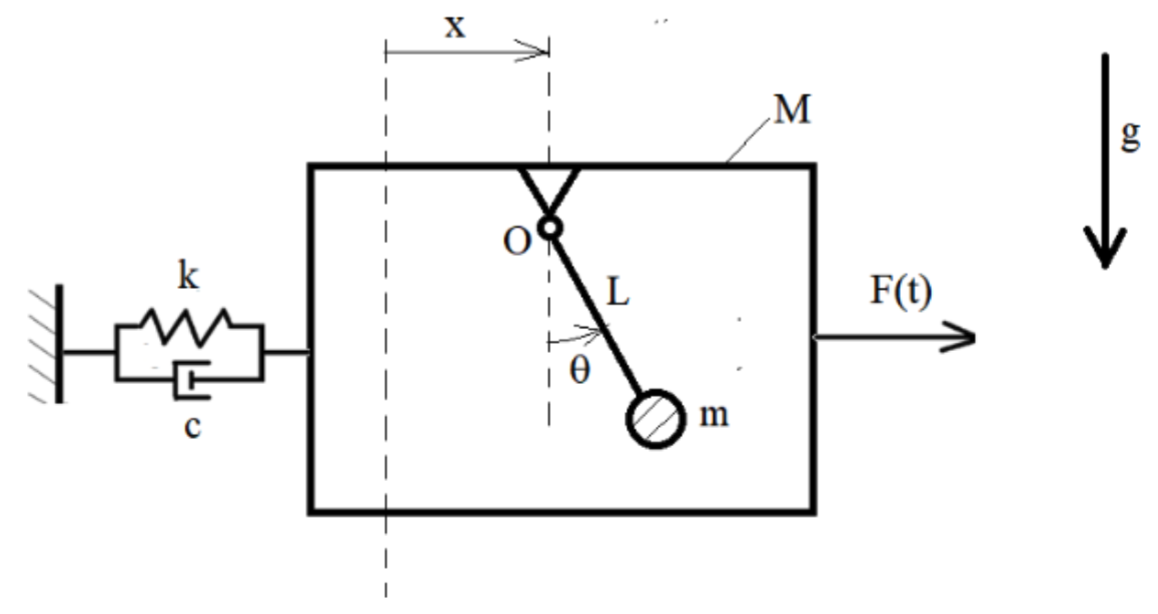
\includegraphics[width=0.5\linewidth]{homework/hw1/assets/hw1_p5.png}
    \end{center}
\end{problem}

\begin{enumerate}[(i)]
\item { % 5(i)
    The velocity vector of the pendulum mass $m$ is 
    \begin{equation}
        \bv{v}_m = ( \dot{x} + L \dot{\theta} \cos\theta ) \hat{\bv{i}} + (L \dot{\theta} \sin\theta ) \hat{\bv{j}}
    \end{equation}
    The kinetic energy of the system is thus 
    \begin{equation}
    \begin{aligned}
        K &= \frac{1}{2} M \dot{x}^2 + \frac{1}{2} m \left[ {\left( \dot{x} + L \dot{\theta} \cos\theta \right)}^2 + {\left( L \dot{\theta} \sin\theta \right)}^2 \right]  \\
        &= \frac{1}{2} (M + m) \dot{x}^2 + \frac{1}{2} m L^2 \dot{\theta}^2 + m L \dot{x} \dot{\theta} \cos\theta
    \end{aligned}
    \end{equation}
    The potential energy, taking into account the gravitational potential energy (setting the natural state $\theta = 0$ as the reference state), is 
    \begin{equation}
        V = \frac{1}{2} k x^2 + m g L (1 - \cos\theta)
    \end{equation}
    where we only consider gravity acting upon $m$ since $M$ is constrained to move horizontally. 

    With respect to $\delta x$ (variation in $x$), the generalized force is $F_g(t) = -c \dot{x}(t) + F(t)$ which consists of the \emph{damping force} and the \emph{imposed external force}. 
    Since gravity is readily accounted for in the potential energy as a conservative field, there is no generalized force acting upon $\delta \theta$.
    Defining $\mathcal{L} = K - V$, the Euler-Lagrange equations read
    \begin{equation}
        \frac{d}{dt} \left( \frac{\partial \mathcal{L}}{\partial \dot{x}} \right) - \frac{\partial \mathcal{L}}{\partial x} = F_g, ~~~~ \frac{d}{dt} \left( \frac{\partial \mathcal{L}}{\partial \dot{\theta}} \right) - \frac{\partial \mathcal{L}}{\partial \theta} = 0
    \end{equation}
    The first equation leads to
    \begin{equation}\label{eqn:hw1_p5_gov_x}
    \begin{aligned}
        &&\left[(M+m)\ddot{x} + \frac{d}{dt}\left(mL\dot{\theta} \cos\theta\right)\right] - \left[-kx\right] &= -c\dot{x} + F(t) \\
        \Rightarrow && \Aboxed{(M+m)\ddot{x} +mL \ddot{\theta} \cos\theta - mL\dot{\theta}^2 \sin\theta + c\dot{x} + kx &= F(t)}
    \end{aligned}
    \end{equation}
    and the second equation yields 
    \begin{equation}\label{eqn:hw1_p5_gov_theta}
    \begin{aligned}
        && \left[mL^2 \ddot{\theta} + \frac{d}{dt}\left(mL\dot{x} \cos\theta\right)\right] - \left[-mL \dot{x} \dot{\theta} \sin\theta - mgL\sin\theta \right] &= 0 \\
        \Rightarrow && \Aboxed{\ddot{x}\cos\theta + L\ddot{\theta} + g\sin\theta &= 0}
    \end{aligned}
    \end{equation}
}
\item { % 5(ii)
    With $F(t) = 0$, the static equilibrium position can be obtained by setting all time derivatives to zero. 
    Then, \cref{eqn:hw1_p5_gov_x,eqn:hw1_p5_gov_theta} become
    \begin{equation}
    \begin{aligned}
        kx = 0 & ~~~~\Rightarrow ~~~~x = 0 \\
        g\sin\theta = 0 & ~~~~\Rightarrow ~~~~\theta = 0
    \end{aligned}
    \end{equation}
    which confirms that $x = \theta = 0$ is indeed an equilibrium position. 
    Note that $\theta = \pi$ is also an equilibrium, albeit an unstable one (show by linear stability analysis). 
    In this case, physical constraints also dictates that $\theta = \pi$ cannot be a solution as it corresponds to the pendulum being inverted. 

    To linearize the equations about $x = \theta = 0$, we simply Taylor-expand $\sin\theta$ and $\cos\theta$ with respect to $\theta = 0$ and remove all nonlinear terms. 
    The result reads 
    \begin{equation}
    \begin{aligned}
        (M+m)\ddot{x} + mL \ddot{\theta} + c\dot{x} + kx &= 0 \\
        \ddot{x} + L\ddot{\theta} + g\theta &= 0
    \end{aligned}
    \end{equation}
    or in matrix forms,
    \begin{equation}
    \boxed{
        \begin{bmatrix} M+m & mL \\ 1 & L \end{bmatrix}
        \begin{bmatrix} \ddot{x} \\ \ddot{\theta} \end{bmatrix}
        + 
        \begin{bmatrix} c & 0 \\ 0 & 0\end{bmatrix}
        \begin{bmatrix} \dot{x} \\ \dot{\theta}\end{bmatrix}
        + 
        \begin{bmatrix} k & 0 \\ 0 & g \end{bmatrix}
        \begin{bmatrix} x \\ \theta \end{bmatrix} = 0
    }.
    \end{equation}
}
\end{enumerate}

